% !TeX root = ../main.tex
% Add the above to each chapter to make compiling the PDF easier in some editors.

\chapter{Methodology}\label{chapter:methodology}

\section{Terminology}
\label{sec:terminology}

Before we dive into technical explanations, we want to clear some potential terminology confusion.

In the original DICE release from Microsoft \cite{England2016}, the identifier of a component is called the Firmware ID (FWID).
The TCG consortium later renamed it TCB Component Identifier (TCI).
We believe this is to emphasize that the TCI does not necessarily have to be the hash of a firmware binary, but could also be, for example, the embedded ID of a hardware component.
However, TCG has not fully implemented this terminology renaming.
Their DICE Attestation Architecture \cite{TCGAttestation2020} defines an X.509 extension that contains the TCIs.
They continue to be referred to as FWIDs in the formal definition of this extension, while everywhere else they are referred to as TCIs.
In personal correspondence with TCG, we have learned that this is due to backwards compatibility.
The old term FWID is retained whenever it is used in something that is alive in the long term, like formal definitions, and the new term TCI in assets that can be updated more quickly, such as the specification text.
Therefore, we will use the term TCI in this theoretical chapter, and in the implementation chapter (\autoref{chapter:implementation}) we will use the term FWID, just as it is common practice at the TCG.


\section{Architectural overview}

\begin{figure}[htpb]
  \centering
  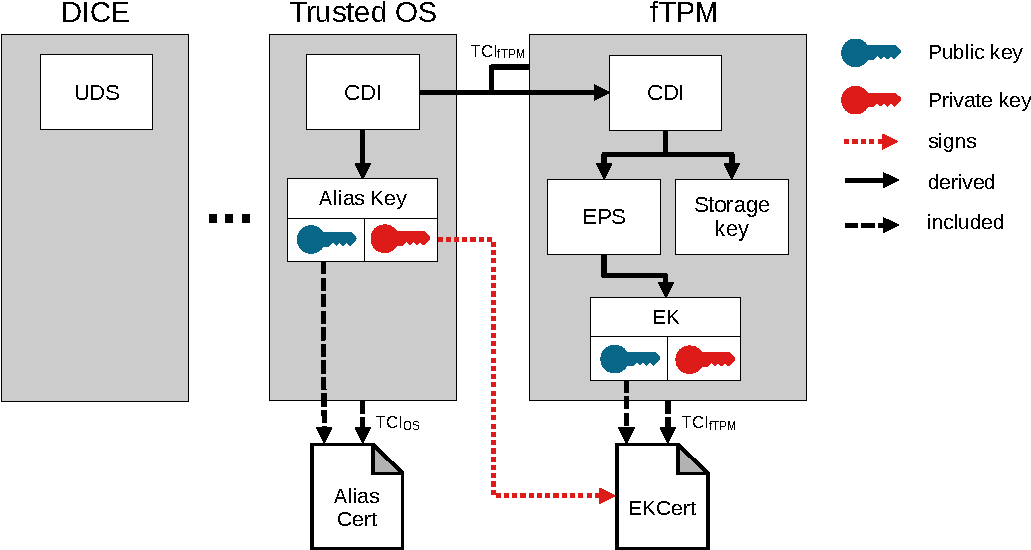
\includegraphics[width=1\linewidth]{figures/architecture.pdf}
  \caption{The architecture of our system.} \label{fig:architecture}
\end{figure}


We have an S-RTM, which uses the consistent trusted state a device has after powering-on for further measurements. This in contrast to D-RTM, which is capable of doing so at anytime, e.g., Intel SGX.
% S-RTM = DICE

% EK = AK: Takes on both roles. Endorsement key always represents identity, therefore, we lose privacy. Later an approach with privacy is presented.
% However, we don't require a privacy CA, but instead trust the manufacturer of our trust anchor directly (DICE), which is sufficient for our approach.

% EK does not represent devices' identity anymore, but DICEs' DeviceCert does.
% Lifetime of EK is bound to the exact software versions of the fTPM including all underlying firmware

% 5.3.2 from https://dl.acm.org/doi/10.1145/3098954.3103165
% Use the references there to explain why we used HMAC with SHA256
% Even though https://trustedcomputinggroup.org/wp-content/uploads/Hardware-Requirements-for-Device-Identifier-Composition-Engine-r78_For-Publication.pdf says hash-only is also an option, https://nvlpubs.nist.gov/nistpubs/SpecialPublications/NIST.SP.800-57pt1r5.pdf (Table 3) shows that the HMAC version has roughly double security strength. Cite all three here (ACM, TCG, NIST)!


% Prover/Verifier (in many earlier papers) vs. Attester/Verifier/Relying Party (RFC)

\section{The identities of an fTPM}

Depending on the point of view, there are two identities of an fTPM.
There is the identity of the fTPM measured by DICE, which consists of the hash of the binary and the component configurations as for all DICE components, as shown in \autoref{fig:ftpm-identity}.
This identity is referred to as the TCI.
Compilation flags are not part of these configurations, as they are embedded in the final binary and are therefore automatically measured as part of the measurement of the binary.
Of more interest are the configurations that are not part of the binary.
They are usually provided in well-known formats such as \texttt{json} or \texttt{xml}.
However, Microsoft's fTPM reference implementation does not contain such configurations, which simplifies the TCI generation of our fTPM by limiting it to the measurement of the fTPM binary data.
The TPM's storage cannot be part of its identity as it changes during runtime after each data write, e.g., storing an arbitrary key.
This is a problem because DICE only runs during the boot time in which the identity of the fTPM is measured.
The identity of the fTPM must not change afterwards, otherwise the consistency of the identity transmitted by DICE and the actual identity of the fTPM would differ.
In the interest of completeness, we also do not want to restrict the permissible values of the working data of an fTPM.

Then, there is also the identity of the fTPM in the TPM context, which is represented by its EK.
This identity is not only bound to the binary and the configuration of the fTPM, but also the entire underlying firmware stack.
We derive the EK from the TPMs CDI, which is derived of the measurements of all preceding firmware components and the TPMs' TCI, see \autoref{eq:dice_cdi}.
A TPMs storage must never be accessible to another TPM.
Therefore, if the TPMs identity changes, e.g., due to a TPM modification or an update of a preceding firmware component, the old storage data is inaccessible, which is equivalent to a full manufacturer reset.


\begin{figure}[htpb]
  \centering
  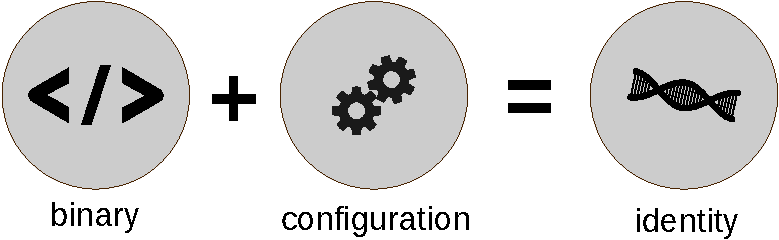
\includegraphics[width=0.6\linewidth]{figures/ftpm-identity.pdf}
  \caption{The accumulation of the binary and its configuration to its identity.} \label{fig:ftpm-identity}
\end{figure}


% In the context of DICE, the identity of a firmware component generally consists of the binary and its configuration, as depicted in \autoref{fig:ftpm-identity}.


% Configurations required
% Does contain whole firmware stack?
% Data cannot be considered, since changes during runtime, not represented by DICE which only happens at boot-time
% What happens if identity changed? -> Data not accessible, in essence, fTPM fully reset
% https://trustedfirmware-a.readthedocs.io/en/latest/design_documents/measured_boot.html#critical-data


\section{Chaining DICE and TPM certificate infrastructure}

\section{Provisioning process}

% To summarize, attestation key provisioning must ensure that only valid attestation key material is established in Attesters [RFC 9334]

\section{Attestation process}

% Check also for revocation of manufacturer cert

\begin{equation}
trusted(C_{i}) \, \coloneqq \, \bigwedge_{k=0}^{i} trusted(C_{k})
\end{equation}

% We use explicit attestation. See DICE Layering Spec 7.2
% See 8.1.1.2 for an example about implicit attestation
% Implicit attestation would require to know all resulting public keys in EKcert, which would require that we booted it up in a controlled manner beforehand and stored the resulting code.
We use an explicit attestation procedure.
This makes it sufficient for the verifier to know the trusted TCI, whereas implicit attestation would require a database of known public keys corresponding to a trusted TCI.
And since each public key for a device is unique, as it is ultimately derived from the device's unique UDS, the verifier would need to know the mapping between public keys and the corresponding TCI for each device, which we consider unrealistic.
Also, this is a hindrance as the verifier should be able to trust an unknown device by trusting the DICE manufacturer.

\section{Updating the fTPM}

We consider it as critical that the \ac{fTPM} is updatable. This is due to the history of \acp{fTPM} showing vulnerabilities which have been patched consequently. % cite... all from background probably

Our \ac{fTPM} can be only updated with the system shut down. This is due to the required out-of-band signing procedure of trusted applications before being deployed. This also  with while system is shut down. This ensures that the TCI part of the EKcert generated at boot-time does not become obsolete, in other words, keeps representing the state of the currently running fTPM.

% Clear data

To protect against downgrade attacks:
NV data is encrypted/integrity with AESP
Encryption required to ensure confidentiality
AESP used to also ensure integrity
This is required since also the cipher text of the NV could be modified, which might change security critical information.
Encryption-only would not prohibit that.
As soon as an integrity violation is detected, the \ac{fTPM} is fully reset, effectively invalidating all previously stored data.
Note that an attacker could thereby easily trigger a data loss.
This has to avoided by integrating the good-practices with working with a \ac{TPM}, which includes having secrets stored also elsewhere. % Maybe cite something, I feel like Microsoft has something for that
This introduces storage and memory overhead.
Processing overhead only slightly, since the data is already decrypted during start-time, which happens only once at boot time, and then later data is encrypted only while it is stored, which happens only ... % TODO: When s it happen? I remember there were not many places in the code where storing of the NV onto the persistent storage is triggered. 
Hence, there is no performance penalty during common uses of a \ac{TPM}, e.g., key creation.

% Add layered figure which shows that the hard drive never sees decrypted data, but only the secure memory. Important because data can be stored in NW.
This might seem redundant because of the storage protection of for example TrustZone, but this does not protect against downgrade attacks. With our approach, the access to the data is bound to the exact identity of the fTPM including all underlying firmware.

So, our protection additionally protects data-at-rest, while the data-at-use is protected by the TEE's secure memory, i.e., the memory isolation from the normal world.



\section{Privacy}

% General: Contradiction
% Goal of DICE is explicitly to establish a long-term identity. So, we need to work against its design.

% Maybe: The certificates would need to be encrypted as well, as they contain the TCI values, potentially identifying the device

% Use Attestation key not in endorsement (or platform?) hierarchy

% Each AliasKey is a identity key as specified in DICE layering Architecture 8.1.1.5
% They would need to be made independent of the devices identity.
